\documentclass[11pt,a4paper]{article}
\usepackage[utf8]{inputenc}
\usepackage[T1]{fontenc}
\usepackage{lmodern}
\usepackage{amsmath,amssymb,amsthm}
\usepackage{booktabs}
\usepackage{array}
\usepackage{microtype}
\usepackage[margin=2.5cm]{geometry}
\usepackage{enumitem}
\usepackage{xcolor}
\usepackage{pgfplots}
\pgfplotsset{compat=1.16}
\usepackage[colorlinks=true,linkcolor=blue!60!black,citecolor=blue!60!black,urlcolor=blue!50!black]{hyperref}
\usepackage{url}

\newtheorem{theorem}{Theorem}[section]
\newtheorem{proposition}[theorem]{Proposition}
\newtheorem{lemma}[theorem]{Lemma}
\newtheorem{corollary}[theorem]{Corollary}
\newtheorem{conjecture}[theorem]{Conjecture}
\newtheorem*{thmA}{Theorem A}
\newtheorem*{thmB}{Theorem B}
\newtheorem*{thmC}{Theorem C}
\newtheorem*{corD}{Corollary D}
\theoremstyle{definition}
\newtheorem{definition}[theorem]{Definition}
\newtheorem{problem}[theorem]{Problem}
\theoremstyle{remark}
\newtheorem{remark}[theorem]{Remark}

\newcommand{\R}{\mathbb{R}}
\newcommand{\eps}{\varepsilon}
\newcommand{\av}[1]{\langle #1\rangle}
\newcommand{\Dd}{D_\delta}
\newcommand{\sig}{\sigma_{\mathrm c}}
\newcommand{\eL}{\varepsilon_{\mathrm L}}
\newcommand{\eB}{\varepsilon_{\mathrm B}}
\newcommand{\Lx}{L}
\newcommand{\Vy}{V}

\title{The curvature of the Fisher--Rao beta manifold decreases in both parameters\\[4pt]
\large Defect calculus for Hessian metrics of additive differences\\ and a proof of the Le Brigant--Preston--Puechmorel conjecture}
\author{Research audit XXV\thanks{Manuscript prepared with the assistance of an AI system (Claude, Anthropic). Every computation is reproducible from the scripts and logs in the folder \texttt{xxv/} of the accompanying repository (Appendix~\ref{app:repro}). Author attribution is to be completed by the submitting author.}}
\date{October 29, 2026}

\begin{document}
\maketitle

\begin{abstract}
Let $K(x,y)$ be the sectional curvature of the Fisher--Rao metric on the manifold of beta distributions $\mathrm{Beta}(x,y)$, $x,y>0$. Le Brigant, Preston and Puechmorel showed that $K<0$, and they conjectured that $K>-\tfrac12$; in the form recalled by Qi, the conjecture also asserts that $K$ is decreasing in each parameter. Previously only the diagonal $x=y$ had been settled. We prove the full conjecture: $\partial_xK<0$ and $\partial_yK<0$ on $(0,\infty)^2$, hence $-\tfrac12<K<0$, and both bounds are sharp.

The proof rests on a \emph{defect calculus} for Hessian metrics of additive differences $F(x)+F(y)-F(x+y)$. With $h=1/F''$ and $G=-F''/F'''$ the curvature factorizes as
\[
K(x,y)=-\frac{h'(x)\,h'(y)\,h'(x+y)\,A(x,y)}{4\,B(x,y)^2},
\]
where $A=G(x+y)-G(x)-G(y)$ and $B=h(x+y)-h(x)-h(y)$ are subadditivity defects.
This identity gives four things. It gives a one-line proof of negativity. It gives exact edge laws $K(x,0^+)=-\tfrac12\bigl(G'(x)-\tfrac12\bigr)$ and $K(x,\infty)=-h'(x)\bigl(x-G(x)\bigr)/\bigl(4(x-h(x))^2\bigr)$. It gives a regular averaged formula for $\partial_x\log(-K)$ along the edges. And it gives a \emph{defect balance} identity, $2B-A=\tfrac12+O(\text{argument}^{-3})$, which removes the second-order cancellation at infinity.

For $F=\log\Gamma$, seven one-variable shape lemmas reduce the conjecture to finitely many inequalities in one variable plus one compact two-variable region. There, monotone corner bounds turn positivity on boxes into point evaluations. Every inequality is certified in ball arithmetic (Arb), with Alzer's enveloping series for large arguments; the complete verification runs in about two minutes.

As by-products we obtain the explicit squeeze $\max\{K(x,\infty),K(y,\infty)\}<K(x,y)<\min\{K(x,0^+),K(y,0^+)\}$, strict decrease along rays, and new proofs of the diagonal results of Qi and Qi--Agarwal.
\end{abstract}

\tableofcontents

\section{Introduction}\label{sec:intro}

\subsection{The conjecture}
The beta distributions $\mathrm{Beta}(x,y)$, with density $t^{x-1}(1-t)^{y-1}/B(x,y)$ on $(0,1)$, form a two-parameter exponential family. Their Fisher information is the Hessian of the log-partition function
\[
\varphi(x,y)=\log B(x,y)=\log\Gamma(x)+\log\Gamma(y)-\log\Gamma(x+y),
\]
that is, with $\psi_k=\psi^{(k)}$ the polygamma functions and $s=x+y$,
\begin{equation}\label{eq:metric}
g=\begin{pmatrix}\psi_1(x)-\psi_1(s)&-\psi_1(s)\\-\psi_1(s)&\psi_1(y)-\psi_1(s)\end{pmatrix}.
\end{equation}
The Fisher--Rao geometry of beta and Dirichlet distributions was studied by Le Brigant and Puechmorel \cite{LBP19} and by Le Brigant, Preston and Puechmorel \cite{LBPP21}. They proved that the Dirichlet manifolds are Hadamard manifolds; in particular the sectional curvature $K(x,y)$ of the beta manifold is negative. Explicitly,
\begin{equation}\label{eq:K}
K(x,y)=\frac{\psi_2(s)\bigl[\psi_1(x)\psi_2(y)+\psi_1(y)\psi_2(x)\bigr]-\psi_1(s)\psi_2(x)\psi_2(y)}{4\bigl[\psi_1(x)\psi_1(y)-\psi_1(s)\bigl(\psi_1(x)+\psi_1(y)\bigr)\bigr]^2}.
\end{equation}
From the limiting values and from numerical evidence they conjectured a lower bound \cite{LBPP21}. The conjecture has been recalled in the following form in \cite{QA24,Qi26}.

\begin{conjecture}[Le Brigant--Preston--Puechmorel]\label{conj:LBPP}
The sectional curvature of the Fisher--Rao beta manifold satisfies $K(x,y)>-\frac12$ for all $x,y>0$, and $K(x,y)$ is decreasing in $x$ and in $y$.
\end{conjecture}

The progress so far concerns the diagonal. The sharp bounds $-\tfrac12<K(x,x)<0$ are established in \cite{Qi21,QA24} through complete monotonicity of functions built from polygamma functions. In September 2026 Qi \cite{Qi26} proved that $x\mapsto K(x,x)$ is strictly decreasing. The two-variable statement remained open: it is recalled as a conjecture in \cite{Qi26}, and the survey of open problems \cite[§R2]{VMRC} lists it in October 2026 among the problems not attempted. The methods used on the diagonal (Laplace transforms, Bernstein's theorem) are one-dimensional, while $K$ depends on two variables through three polygamma arguments $x$, $y$, $x+y$.

\subsection{Results}
We write $h=1/\psi_1$ and $G=-\psi_1/\psi_2$ (so $G=h/h'$), and
\[
g(z)=z-G(z),\qquad e(z)=z-h(z)\qquad(z>0).
\]
Both $g$ and $e$ are increasing, concave, and tend to $0$ at $0^+$ and to $\frac12$ at $\infty$ (Corollary~\ref{cor:derived}).

\begin{thmA}
For all $x,y>0$,
\[
\frac{\partial K}{\partial x}(x,y)<0\qquad\text{and}\qquad\frac{\partial K}{\partial y}(x,y)<0 .
\]
Consequently $-\tfrac12<K(x,y)<0$ on $(0,\infty)^2$. Moreover $K(x,y)\to-\tfrac12$ as $\min(x,y)\to\infty$ and $K(x,y)\to0$ as $x+y\to0$, so both bounds are sharp. Conjecture~\ref{conj:LBPP} is true.
\end{thmA}

\begin{thmB}[edge laws and squeeze]
For every $x>0$ the limits
\[
K_0(x):=\lim_{y\to0^+}K(x,y)=-\frac{G'(x)-\frac12}{2},\qquad K_\infty(x):=\lim_{y\to\infty}K(x,y)=-\frac{h'(x)\,g(x)}{4\,e(x)^2}
\]
exist. $K_0$ is a strictly decreasing bijection of $(0,\infty)$ onto $(-\frac14,0)$, and $K_\infty$ is a strictly decreasing bijection onto $(-\frac12,-\frac14)$. For all $x,y>0$,
\[
\max\{K_\infty(x),K_\infty(y)\}<K(x,y)<\min\{K_0(x),K_0(y)\}.
\]
\end{thmB}

\begin{thmC}[defect calculus]
Let $F\in C^4(0,\infty)$ with $F''>0>F'''$, put $h=1/F''$, $G=-F''/F'''$, and let $K_F$ be the Gaussian curvature of the Hessian metric of $\Phi(x,y)=F(x)+F(y)-F(x+y)$ wherever the metric is positive definite. Then
\[
K_F(x,y)=-\frac{h'(x)h'(y)h'(x+y)\,A(x,y)}{4B(x,y)^2},
\]
with $A,B$ as in the abstract. The metric is positive definite exactly where $B>0$. Where $A>0$, the logarithmic derivative $q=\partial_x\log(-K_F)$ is given by the raw formula \eqref{eq:raw}, the balance formula \eqref{eq:balance} and, under a mild condition at $0$, by the averaged formula \eqref{eq:avg}.
\end{thmC}

\begin{corD}
The diagonal curvature $x\mapsto K(x,x)$ decreases strictly from $0$ to $-\frac12$ (\cite{Qi26}, \cite{Qi21,QA24}). For every $(x,y)$ the function $\lambda\mapsto K(\lambda x,\lambda y)$ is strictly decreasing on $(0,\infty)$. For $-\frac12<c<0$ each nonempty level set $\{K=c\}$ is the graph of a strictly decreasing smooth function.
\end{corD}

\subsection{A new problem, the method, and the application}
The proof follows a three-step scheme. First, a new problem forces the right structures to appear. Second, a method is developed to solve it. Third, the method is applied to Conjecture~\ref{conj:LBPP}.

\begin{problem}[edge-squeeze problem]\label{prob:edge}
Let $F$ be a strictly convex function on $(0,\infty)$ with $F'''<0$, and let $K_F$ be the curvature of the Hessian metric of $F(x)+F(y)-F(x+y)$. Determine the edge laws $x\mapsto K_F(x,0^+)=\lim_{y\to0^+}K_F(x,y)$ and $x\mapsto K_F(x,\infty)=\lim_{y\to\infty}K_F(x,y)$. Decide whether $K_F(x,y)$ always lies strictly between its two edge values, and whether it is monotone between them.
\end{problem}

For $F=\log\Gamma$, Theorem~B answers Problem~\ref{prob:edge} completely. Since $K_\infty(x)\to-\frac12$ as $x\to\infty$ and $K_\infty>-\frac12$, the squeeze alone already gives the lower bound in Conjecture~\ref{conj:LBPP}. The method has four ingredients.

\begin{enumerate}[label=(\roman*)]
\item \emph{Defect representation} (Theorem~\ref{thm:defect}). The curvature is a quotient of two subadditivity defects, of $G$ and of $h$, weighted by $h'$ at the three arguments. This explains the sign of $K$, gives the edge laws, and reduces all two-variable information to two \emph{one}-variable functions $G$ and $h$.
\item \emph{Averaged representation} (Proposition~\ref{prop:avg}). Writing $A$ and $B$ as averages of $G''$ and $h''$ over the segment family $\alpha x+\beta y$ gives a formula for $\partial_x\log(-K)$ in which the $1/x$ singularities along the edges have cancelled.
\item \emph{Defect balance} (Proposition~\ref{prop:raw}). At infinity $A\approx B\approx\frac12$, but the first-order variations of $A$ and $B$ are locked in the ratio $2:1$: $2B-A=\frac12+O(z^{-3})$. Rewriting $\partial_x\log(-K)$ through $\delta'=G'-2h'+1=O(z^{-4})$ removes the second-order cancellation.
\item \emph{Shape-constrained certification} (Sections~\ref{sec:shape}--\ref{sec:proof}). Seven one-variable shape lemmas (convexity of $h$ and $G$, unimodality of $G''$, signs of $h'''$ and of $2h''-G''$, and so on) make every building block of $\partial_x\log(-K)$ monotone or unimodal in each variable. Positivity on a box then follows from finitely many point values at its corners. Outside a compact region the same lemmas reduce everything to inequalities in one variable.
\end{enumerate}

\subsection{Computer assistance}
The shape lemmas and the remaining finitely many inequalities are verified with interval (ball) arithmetic. We use Arb \cite{Joh17} through python-flint, with exact rational symbolic preprocessing in SymPy. Three exact representations of each polygamma expression are used:
\begin{itemize}
\item an algebraically regularized form near $0$, built from $\psi_k(1+z)$;
\item the plain form on $[1,3]$;
\item Alzer's two-sided enveloping inequalities \cite{Alz97} on $[3,\infty)$, for which we include a short proof (Lemma~\ref{lem:alzer}).
\end{itemize}
No floating-point computation enters a proof. The scripts, the logs and a single command reproducing all certificates in about two minutes are described in Appendix~\ref{app:repro}.

\subsection{Organisation}
Section~\ref{sec:defect} develops the defect calculus for general $F$ (Theorem~C). Section~\ref{sec:shape} contains the polygamma toolkit and the shape lemmas for $F=\log\Gamma$. Section~\ref{sec:proof} proves that $\partial_x\log(-K)>0$ by splitting $(0,\infty)^2$ into six regions. Section~\ref{sec:main} proves Theorems~A and~B and Corollary~D. Section~\ref{sec:remarks} discusses asymptotics, the scope of the method and open questions.

\begin{figure}[t]
\centering
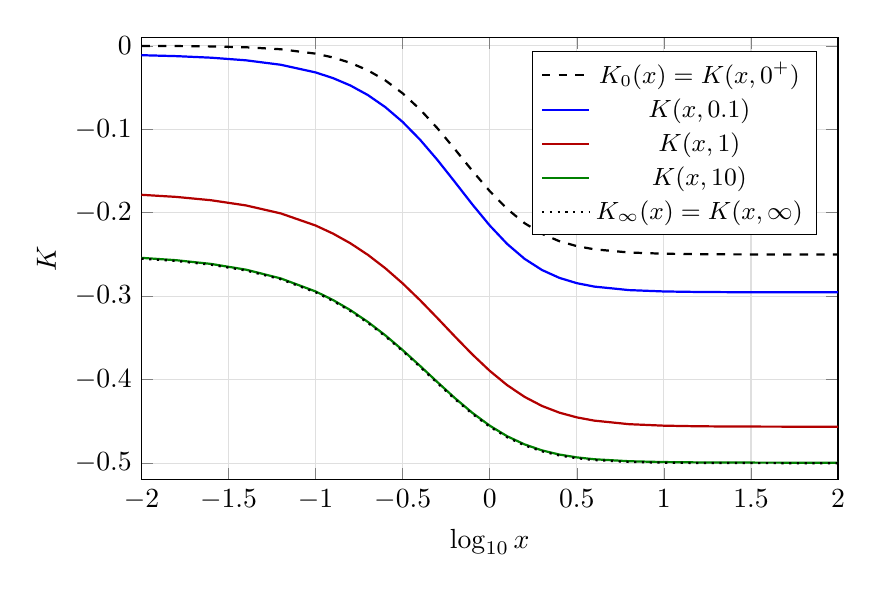
\begin{tikzpicture}
\begin{axis}[width=0.86\textwidth,height=7.2cm,xlabel={$\log_{10}x$},ylabel={$K$},ymin=-0.52,ymax=0.01,xmin=-2,xmax=2,
legend pos=north east,legend style={font=\small},grid=major,grid style={gray!25}]
\addplot[thick,black,dashed] table[x=log10u,y=K0] {
log10u K0
-2.00 -0.000120
-1.80 -0.000296
-1.60 -0.000724
-1.40 -0.001746
-1.20 -0.004118
-1.00 -0.009393
-0.90 -0.013945
-0.80 -0.020406
-0.70 -0.029352
-0.60 -0.041370
-0.50 -0.056936
-0.40 -0.076228
-0.30 -0.098907
-0.20 -0.123950
-0.10 -0.149682
0.00 -0.174095
0.10 -0.195393
0.20 -0.212494
0.30 -0.225220
0.40 -0.234101
0.50 -0.239999
0.60 -0.243780
0.80 -0.247624
1.00 -0.249090
1.20 -0.249648
1.40 -0.249863
1.60 -0.249946
1.80 -0.249979
2.00 -0.249992
};
\addlegendentry{$K_0(x)=K(x,0^+)$}
\addplot[thick,blue] table[x=log10u,y=K] {
log10u K
-2.00 -0.011238
-1.80 -0.012370
-1.60 -0.014239
-1.40 -0.017372
-1.20 -0.022706
-1.00 -0.031881
-0.90 -0.038698
-0.80 -0.047566
-0.70 -0.058979
-0.60 -0.073417
-0.50 -0.091240
-0.40 -0.112520
-0.30 -0.136853
-0.20 -0.163217
-0.10 -0.190000
0.00 -0.215292
0.10 -0.237379
0.20 -0.255211
0.30 -0.268594
0.40 -0.278027
0.50 -0.284355
0.60 -0.288453
0.80 -0.292666
1.00 -0.294292
1.20 -0.294916
1.40 -0.295157
1.60 -0.295251
1.80 -0.295288
2.00 -0.295302
};
\addlegendentry{$K(x,0.1)$}
\addplot[thick,red!70!black] table[x=log10u,y=K] {
log10u K
-2.00 -0.178486
-1.80 -0.181027
-1.60 -0.185011
-1.40 -0.191220
-1.20 -0.200792
-1.00 -0.215292
-0.90 -0.224978
-0.80 -0.236611
-0.70 -0.250389
-0.60 -0.266422
-0.50 -0.284656
-0.40 -0.304809
-0.30 -0.326308
-0.20 -0.348291
-0.10 -0.369688
0.00 -0.389403
0.10 -0.406538
0.20 -0.420581
0.30 -0.431463
0.40 -0.439485
0.50 -0.445153
0.60 -0.449026
0.80 -0.453296
1.00 -0.455088
1.20 -0.455816
1.40 -0.456109
1.60 -0.456226
1.80 -0.456273
2.00 -0.456291
};
\addlegendentry{$K(x,1)$}
\addplot[thick,green!50!black] table[x=log10u,y=K] {
log10u K
-2.00 -0.254029
-1.80 -0.256874
-1.60 -0.261316
-1.40 -0.268189
-1.20 -0.278674
-1.00 -0.294292
-0.90 -0.304548
-0.80 -0.316676
-0.70 -0.330772
-0.60 -0.346802
-0.50 -0.364537
-0.40 -0.383505
-0.30 -0.402977
-0.20 -0.422029
-0.10 -0.439679
0.00 -0.455088
0.10 -0.467739
0.20 -0.477523
0.30 -0.484689
0.40 -0.489701
0.50 -0.493083
0.60 -0.495310
0.80 -0.497687
1.00 -0.498677
1.20 -0.499098
1.40 -0.499280
1.60 -0.499360
1.80 -0.499395
2.00 -0.499410
};
\addlegendentry{$K(x,10)$}
\addplot[thick,black,dotted] table[x=log10u,y=Kinf] {
log10u Kinf
-2.00 -0.254952
-1.80 -0.257803
-1.60 -0.262256
-1.40 -0.269147
-1.20 -0.279657
-1.00 -0.295312
-0.90 -0.305591
-0.80 -0.317746
-0.70 -0.331872
-0.60 -0.347933
-0.50 -0.365699
-0.40 -0.384695
-0.30 -0.404191
-0.20 -0.423256
-0.10 -0.440908
0.00 -0.456304
0.10 -0.468929
0.20 -0.478676
0.30 -0.485795
0.40 -0.490755
0.50 -0.494082
0.60 -0.496253
0.80 -0.498521
1.00 -0.499420
1.20 -0.499772
1.40 -0.499910
1.60 -0.499964
1.80 -0.499986
2.00 -0.499994
};
\addlegendentry{$K_\infty(x)=K(x,\infty)$}
\end{axis}
\end{tikzpicture}
\caption{The curvature $K(x,y)$ as a function of $\log_{10}x$ for $y=0.1,1,10$, together with the edge laws $K_0$ and $K_\infty$ of Theorem~B. Every curve decreases, and the curves are ordered as $y$ increases. The value $K(x,y)\to K_\infty(y)$ as $x\to\infty$, for example $K(\infty,0.1)=K_\infty(0.1)=-0.2953\ldots$. Data: \texttt{data/plot\_K.dat}; illustration only.}\label{fig:K}
\end{figure}

\section{Defect calculus for Hessian metrics of additive differences}\label{sec:defect}

\subsection{Curvature of a two-dimensional Hessian metric}
\begin{lemma}\label{lem:hessian}
Let $\Phi\in C^4(U)$, $U\subset\R^2$ open, with positive definite Hessian $g=\nabla^2\Phi$, and write $\Phi_{ij}$, $\Phi_{ijk}$ for partial derivatives and $D=\det g$. The Gaussian curvature of $g$ is
\[
K=\frac{R_{1212}}{D},\qquad R_{1212}=\frac14\sum_{p,q}g^{pq}\bigl(\Phi_{12p}\Phi_{12q}-\Phi_{11p}\Phi_{22q}\bigr),
\]
equivalently
\[
K=-\frac{\det M}{4D^2},\qquad M=\begin{pmatrix}\Phi_{11}&\Phi_{12}&\Phi_{22}\\\Phi_{111}&\Phi_{112}&\Phi_{122}\\\Phi_{112}&\Phi_{122}&\Phi_{222}\end{pmatrix}.
\]
\end{lemma}
\begin{proof}
For a Hessian metric the Christoffel symbols of the first kind are $\Gamma_{ij,k}=\frac12\Phi_{ijk}$. In the classical expression
\[
R_{1212}=-\tfrac12\bigl(g_{11,22}-2g_{12,12}+g_{22,11}\bigr)+g^{pq}\bigl(\Gamma_{12,p}\Gamma_{12,q}-\Gamma_{11,p}\Gamma_{22,q}\bigr),\qquad K=R_{1212}/D,
\]
the second-derivative part is $-\frac12(\Phi_{1122}-2\Phi_{1122}+\Phi_{1122})=0$. This leaves the stated quadratic expression in third derivatives \cite[Ch.~2]{Shi07}. Expanding $g^{pq}=(\mathrm{adj}\,g)^{pq}/D$ turns $R_{1212}/D$ into $-\det M/(4D^2)$. Both identities were also checked symbolically, together with Brioschi's formula for the Gaussian curvature of $E=\Phi_{11}$, $F=\Phi_{12}$, $G=\Phi_{22}$ (log \texttt{01}).
\end{proof}

For the beta manifold $\Phi=\varphi$, we have $\varphi_{11}=\psi_1(x)-\psi_1(s)$, $\varphi_{12}=-\psi_1(s)$ and $\varphi_{22}=\psi_1(y)-\psi_1(s)$, and the third derivatives are obtained by replacing $\psi_1$ by $\psi_2$. Lemma~\ref{lem:hessian} then gives \eqref{eq:K}.

\subsection{The defect representation}
Let $F\in C^4(0,\infty)$ with $F''>0>F'''$ and put
\[
\psi_1:=F'',\quad \psi_2:=F''',\quad h:=\frac1{\psi_1},\quad G:=-\frac{\psi_1}{\psi_2}=\frac{h}{h'} .
\]
Then $h'=-\psi_2/\psi_1^2>0$. For $x,y>0$ and $s=x+y$ define the \emph{defects}
\[
A(x,y)=G(s)-G(x)-G(y),\qquad B(x,y)=h(s)-h(x)-h(y).
\]

\begin{theorem}[defect representation]\label{thm:defect}
Let $\Phi(x,y)=F(x)+F(y)-F(x+y)$. The Hessian of $\Phi$ is positive definite at $(x,y)$ if and only if $B(x,y)>0$, and there
\begin{equation}\label{eq:defect}
K_F(x,y)=-\frac{h'(x)\,h'(y)\,h'(s)\,A(x,y)}{4\,B(x,y)^2}.
\end{equation}
In particular $\operatorname{sign}K_F=-\operatorname{sign}A$.
\end{theorem}

\begin{proof}
Write $p_k=\psi_k(x)$, $q_k=\psi_k(y)$, $r_k=\psi_k(s)$. Then $\Phi_{11}=p_1-r_1>0$, because $\psi_1$ is decreasing. The determinant is
\[
D=p_1q_1-r_1(p_1+q_1)=p_1q_1r_1\Bigl(\frac1{r_1}-\frac1{p_1}-\frac1{q_1}\Bigr)=p_1q_1r_1\,B,
\]
which gives the first claim. The matrix $M$ of Lemma~\ref{lem:hessian} has rows $(p_1-r_1,-r_1,q_1-r_1)$, $(p_2-r_2,-r_2,-r_2)$, $(-r_2,-r_2,q_2-r_2)$, and a direct expansion gives
\[
-\det M=r_2(p_1q_2+q_1p_2)-r_1p_2q_2=p_2q_2r_2\Bigl(\frac{p_1}{p_2}+\frac{q_1}{q_2}-\frac{r_1}{r_2}\Bigr)=p_2q_2r_2\,A .
\]
Hence $K_F=p_2q_2r_2A/(4p_1^2q_1^2r_1^2B^2)$. Since $p_2/p_1^2=-h'(x)$, $q_2/q_1^2=-h'(y)$ and $r_2/r_1^2=-h'(s)$, this is \eqref{eq:defect}.
\end{proof}

\begin{corollary}[negativity]\label{cor:neg}
Suppose $h$ and $G$ extend continuously to $0$ with $h(0)=G(0)=0$, and $h$, $G$ are strictly convex. Then $A>0$, $B>0$ and $K_F<0$ on $(0,\infty)^2$, and
\begin{equation}\label{eq:double}
A=\int_0^x\!\!\int_0^y G''(a+b)\,db\,da,\qquad B=\int_0^x\!\!\int_0^y h''(a+b)\,db\,da .
\end{equation}
\end{corollary}
\begin{proof}
By the fundamental theorem of calculus, $\int_0^x\int_0^yG''(a+b)\,db\,da=G(s)-G(x)-G(y)+G(0)$. The integrand is positive.
\end{proof}

For the beta manifold the hypotheses hold by Lemma~\ref{lem:small} and Theorem~\ref{thm:shape} (S1, S3). Corollary~\ref{cor:neg} therefore gives a short proof of the negativity theorem of \cite{LBP19,LBPP21} in dimension two, modulo the shape lemmas.

\subsection{The logarithmic derivative}
Assume $A,B>0$ and put
\[
q(x,y):=\partial_x\log\bigl(-K_F(x,y)\bigr),\qquad T(z):=\frac{h''(z)}{h'(z)},\qquad R(z):=T(z)-\frac1z .
\]
Since $-K_F>0$, we have $\partial_xK_F<0$ if and only if $q>0$. We use the increments
\[
\Delta G'=G'(s)-G'(x),\qquad \Delta h'=h'(s)-h'(x),\qquad \Dd=\delta'(x)-\delta'(s),\qquad \delta(z):=G(z)-2h(z)+z .
\]

\begin{proposition}[raw and balance formulas]\label{prop:raw}
\begin{align}
q&=T(x)+T(s)+\frac{\Delta G'}{A}-\frac{2\Delta h'}{B},\label{eq:raw}\\
q&=T(x)+T(s)-\frac{\Dd}{A}+\frac{2\Delta h'\,(B-A)}{AB}.\label{eq:balance}
\end{align}
Moreover $2B-A=\delta(x)+\delta(y)-\delta(s)$.
\end{proposition}
\begin{proof}
By \eqref{eq:defect}, $\log(-K_F)=\log h'(x)+\log h'(y)+\log h'(s)+\log A-2\log B-\log4$, and $\partial_xA=\Delta G'$, $\partial_xB=\Delta h'$; this gives \eqref{eq:raw}. Since $G'=2h'-1+\delta'$, we have $\Delta G'=2\Delta h'-\Dd$, so
\[
\frac{\Delta G'}{A}-\frac{2\Delta h'}{B}=-\frac{\Dd}{A}+2\Delta h'\Bigl(\frac1A-\frac1B\Bigr),
\]
which gives \eqref{eq:balance}. Finally $2B-A=-[(G-2h)(s)-(G-2h)(x)-(G-2h)(y)]=\delta(x)+\delta(y)-\delta(s)$, because $z\mapsto z$ is additive.
\end{proof}

\begin{remark}[why ``balance'']\label{rem:balance}
For $F=\log\Gamma$ we have $\delta(z)=\frac12-\frac{11}{360}z^{-3}+O(z^{-4})$ (Lemma~\ref{lem:alzer}). Hence $2B-A=\frac12+O(\min(x,y)^{-3})$, while $A$ and $B$ themselves differ from $\frac12$ by terms of order $1/\min(x,y)$. In \eqref{eq:raw} the two defect terms are each of order $x^{-2}$ and cancel to leading order. In \eqref{eq:balance} no such cancellation remains: $\Dd=O(x^{-4})$, and the last term is $O(x^{-3})$ and positive.
\end{remark}

\begin{proposition}[averaged formula]\label{prop:avg}
Suppose $h,G\in C^3[0,\infty)$ with $h(0)=G(0)=0$, and $A,B>0$. Define
\[
\av{f}(x,y)=\int_0^1\!\!\int_0^1 f(\alpha x+\beta y)\,d\beta\,d\alpha,\qquad \av{\alpha f}(x,y)=\int_0^1\!\!\int_0^1 \alpha\, f(\alpha x+\beta y)\,d\beta\,d\alpha .
\]
Then $A=xy\av{G''}$, $B=xy\av{h''}$, and
\begin{equation}\label{eq:avg}
q=R(x)+T(s)+\frac{\av{\alpha G'''}}{\av{G''}}-\frac{2\av{\alpha h'''}}{\av{h''}} .
\end{equation}
\end{proposition}
\begin{proof}
Substituting $a=\alpha x$ and $b=\beta y$ in \eqref{eq:double} gives $A=xy\av{G''}$ and $B=xy\av{h''}$. Hence $\partial_x\log A=\frac1x+\av{\alpha G'''}/\av{G''}$ (differentiation under the integral sign), and similarly for $B$. Insert these into $q=T(x)+T(s)+\partial_x\log A-2\partial_x\log B$.
\end{proof}

In \eqref{eq:avg} the terms $T(x)$, $\partial_x\log A$ and $-2\partial_x\log B$, which are each of size $1/x$ near the edge $x=0$, have been combined. Every remaining term is regular up to $x=0$.

\section{Polygamma toolkit and shape lemmas}\label{sec:shape}
From now on $F=\log\Gamma$, so $\psi_k=\psi^{(k)}$ and $h=1/\psi_1$, $G=-\psi_1/\psi_2$. We use the functions
\[
T=\frac{h''}{h'},\quad R=T-\frac1z,\quad g=z-G,\quad e=z-h,\quad \hat g=\tfrac12-g,
\]
\[
\delta'=G'-2h'+1,\quad \eps=2h''-G''=-\delta'',\quad \kappa=G-h .
\]
Each of these is a rational function of $z$ and $\psi_1(z),\dots,\psi_7(z)$, obtained by exact symbolic differentiation with $\psi_k'=\psi_{k+1}$ (script \texttt{symforms.py}).

\subsection{Three exact representations}
\begin{lemma}[regular form near $0$]\label{lem:small}
Put $P_k(z)=\psi_k(1+z)$, which is analytic on $(-1,\infty)$. Then $\psi_k(z)=(-1)^{k+1}k!\,z^{-k-1}+P_k(z)$. In particular
\[
h(z)=\frac{z^2}{1+z^2P_1(z)},\qquad G(z)=\frac{z\,(1+z^2P_1(z))}{2-z^3P_2(z)},
\]
so $h$ and $G$ are analytic in a neighbourhood of $[0,\infty)$, with $h(0)=h'(0)=0$, $h''(0)=2$, $G(0)=0$, $G'(0)=\frac12$, $G''(0)=0$ and $G'''(0)=3\zeta(2)$. More generally, every quantity $Q$ above can be written exactly as $Q=z^{a}\,n(z,P_1,\dots,P_7)/d(z,P_1,\dots,P_7)$, with polynomials $n$, $d$ in $z$ and the $P_k$, $a\in\mathbb Z$, and $n(0,\cdot),d(0,\cdot)\not\equiv0$.
\end{lemma}
\begin{proof}
Use the recurrence $\psi_k(z)=\psi_k(z+1)+(-1)^{k+1}k!z^{-k-1}$, clear denominators, and cancel the largest common power of $z$. The last step is exact polynomial algebra in the independent symbols $z,P_1,\dots,P_7$.
\end{proof}

\begin{lemma}[enveloping expansion; Alzer \cite{Alz97}]\label{lem:alzer}
For integers $k\ge1$, $n\ge0$ and real $z>0$ there is $\theta\in(0,1)$ such that
\[
(-1)^{k+1}\psi_k(z)=S_{k,n}(1/z)+\theta\,E_{k,n}(1/z),
\]
where
\[
S_{k,n}(w)=(k-1)!\,w^k+\tfrac{k!}2\,w^{k+1}+\sum_{j=1}^{n}\frac{B_{2j}\,(2j+k-1)!}{(2j)!}\,w^{2j+k},
\]
\[
E_{k,n}(w)=\frac{B_{2n+2}\,(2n+k+1)!}{(2n+2)!}\,w^{2n+k+2}.
\]
\end{lemma}
\begin{proof}
From the partial-fraction expansion of $\coth$,
\[
\frac t2\coth\frac t2=1+\sum_{m\ge1}\frac{2t^2}{t^2+4\pi^2m^2}.
\]
With $y_m=t^2/(4\pi^2m^2)$ we have $y_m/(1+y_m)=\sum_{i=1}^n(-1)^{i-1}y_m^i+(-1)^ny_m^{n+1}/(1+y_m)$. Summing over $m$ and using $\sum_m2(2\pi m)^{-2i}=(-1)^{i+1}B_{2i}/(2i)!$ gives, for $t>0$,
\[
\frac t2\coth\frac t2=\sum_{i=0}^n\frac{B_{2i}t^{2i}}{(2i)!}+\vartheta_n(t)\frac{B_{2n+2}t^{2n+2}}{(2n+2)!},\qquad\vartheta_n(t)\in(0,1).
\]
Now $(-1)^{k+1}\psi_k(z)=\int_0^\infty t^{k-1}e^{-zt}\,\frac{t}{1-e^{-t}}\,dt$, and $\frac t{1-e^{-t}}=\frac t2+\frac t2\coth\frac t2$. Integrate term by term using $\int_0^\infty t^{k-1+j}e^{-zt}dt=(k-1+j)!\,z^{-k-j}$. The remainder is a positive multiple of $B_{2n+2}$, of absolute value smaller than the corresponding term, because the kernel is positive and $\vartheta_n\in(0,1)$.
\end{proof}

Substituting Lemma~\ref{lem:alzer} with $n=4$ into a quantity $Q$ and expanding exactly in $w=1/z$ and the parameters $\theta_1,\dots,\theta_7\in[0,1]$, one for each $\psi_k$, gives $Q=w^m\,\tilde n(w,\theta)/\tilde d(w,\theta)$ with explicit rational polynomials. For every quantity used below, the lowest power of $w$ in $\tilde n$ and in $\tilde d$ occurs only in the $\theta$-free part. The leading behaviour is therefore exact, for instance
\[
h''\sim\tfrac16z^{-3},\quad h'''\sim-\tfrac12z^{-4},\quad G''\sim\tfrac13z^{-3},\quad G'''\sim-z^{-4},
\]
\[
\eps\sim\tfrac{11}{30}z^{-5},\quad \eps'\sim-\tfrac{11}6z^{-6},\quad \kappa'\sim-\tfrac1{12}z^{-2},\quad \delta'\sim\tfrac{11}{120}z^{-4}.
\]
These leading terms show that the expansions vanish to high order; in $\eps$ the two leading orders of $2h''$ and $G''$ cancel.

\subsection{Certified evaluation}
A quantity $Q$ is enclosed on an interval $[a,b]$ in one of three ways:
\begin{itemize}
\item on $(0,1]$, by the regular form of Lemma~\ref{lem:small}, with $P_k$ enclosed through the Hurwitz zeta function at the ball $1+[a,b]$;
\item on $[1,3]$, by the direct rational form, with $\psi_k(z)=(-1)^{k+1}k!\,\zeta(k+1,z)$ enclosed in Arb;
\item on $[3,\infty]$, by the enveloping form with $w\in[1/b,1/a]$ and $\theta_k\in[0,1]$.
\end{itemize}
All arithmetic is midpoint--radius ball arithmetic at 256 bits; a ball comparison is accepted only if it is certain. To certify a sign on an interval, the interval is cut at $1$ and $3$ and bisected (geometrically on long ranges) until every piece has a certified sign. Since $z^a>0$ and $w^m>0$, the sign of $Q$ on a piece is $\operatorname{sign}(n)\operatorname{sign}(d)$ (respectively $\operatorname{sign}(\tilde n)\operatorname{sign}(\tilde d)$) whenever both are certain. A consistency check of all three forms against high-precision \texttt{mpmath} values is in log \texttt{02}.

\subsection{The shape lemmas}
\begin{theorem}[shape lemmas]\label{thm:shape}
On $(0,\infty)$:
\begin{enumerate}[label=\textup{(S\arabic*)},leftmargin=3.2em]
\item $h''>0$;
\item $h'''<0$;
\item $G''>0$;
\item $G''''<0$ on $(0,\frac25]$, $G'''<0$ on $[\frac3{10},\infty)$ and $G'''>0$ on $(0,\frac{29}{100}]$;
\item $\eps=2h''-G''>0$;
\item $\eps'=2h'''-G'''<0$;
\item $\kappa'=G'-h'<0$ on $[1,\infty)$ and $\kappa>0$ on $(0,1]$.
\end{enumerate}
\end{theorem}
\begin{proof}
Each statement is a sign condition on an explicit quantity. It was certified by the procedure of the previous subsection (script \texttt{lemmas1d.py}, log \texttt{03}); the numbers of certified pieces are listed in Table~\ref{tab:shape}.
\end{proof}

\begin{table}[ht]
\centering
\begin{tabular}{llr}
\toprule
lemma & statement & pieces\\
\midrule
S1 & $h''>0$ on $(0,\infty)$ & 301\\
S2 & $h'''<0$ on $(0,\infty)$ & 1\,020\\
S3 & $G''>0$ on $(0,\infty)$ & 1\,562\\
S4 & $G''''<0$ on $(0,\frac25]$; $G'''<0$ on $[\frac3{10},\infty)$; $G'''>0$ on $(0,\frac{29}{100}]$ & 41; 8\,395; 41\\
S5 & $2h''-G''>0$ on $(0,\infty)$ & 10\,835\\
S6 & $2h'''-G'''<0$ on $(0,\infty)$ & 34\,824\\
S7 & $G'-h'<0$ on $[1,\infty)$; $G-h>0$ on $(0,1]$ & 962; 10\\
\bottomrule
\end{tabular}
\caption{Certified shape lemmas: number of interval pieces in the final partitions (ball arithmetic, 256 bits; total time 51\,s).}\label{tab:shape}
\end{table}

\begin{corollary}\label{cor:derived}
\begin{enumerate}[label=\textup{(\alph*)}]
\item $h'>0$, $h'(0^+)=0$, $h'(\infty)=1$, hence $0<h'<1$. The function $e=z-h$ is increasing and concave, with $e(0^+)=0$ and $e(\infty)=\frac12$, so $0<e<\frac12$. The function $e'=1-h'$ is decreasing. Moreover $h(z)<z^2$.
\item $G'(0^+)=\frac12$ and $G'(\infty)=1$, hence $\frac12<G'<1$. The function $g=z-G$ is increasing and concave, with $g(0^+)=0$ and $g(\infty)=\frac12$, so $0<g<\frac12$. The functions $g'$ and $\hat g=\frac12-g$ are decreasing.
\item $T$ is strictly decreasing.
\item $\delta'$ is strictly decreasing with $\delta'(\infty)=0$, so $\delta'>0$; $\eps$ is positive and strictly decreasing.
\item There is $x_m\in(\frac{29}{100},\frac3{10})$ such that $G''$ is strictly increasing on $(0,x_m]$ and strictly decreasing on $[x_m,\infty)$.
\item $\kappa>0$ on $(0,\infty)$, $\kappa$ is decreasing on $[1,\infty)$, and $\kappa(\infty)=0$.
\item For fixed $y>0$, $x\mapsto\Delta G'(x,y)=G'(x+y)-G'(x)$ is first increasing and then decreasing (possibly only one of the two). In particular, on every interval its minimum is attained at an endpoint.
\end{enumerate}
\end{corollary}
\begin{proof}
The limits at $0$ follow from the regular forms of Lemma~\ref{lem:small}. The limits at $\infty$ follow from Lemma~\ref{lem:alzer} applied to each $\psi_k$ separately, inserted into the exact rational expressions for $h,h',G,G',\dots$; no asymptotic series has to be differentiated term by term. This gives, for example, $h=z-\frac12+\frac1{12z}+O(z^{-2})$, $h'=1+O(z^{-2})$, $G=z-\frac12+\frac1{6z}+O(z^{-2})$ and $G'=1+O(z^{-2})$.

(a) $h'=-\psi_2/\psi_1^2>0$. By S1, $h'$ increases from $0$ to $1$, and $e''=-h''<0$. The bound $h(z)<z^2$ holds because $\psi_1(z)>z^{-2}$.

(b) follows in the same way from S3.

(c) $T'=(h'''h'-h''^2)/h'^2<0$ by S1 and S2.

(d) $\delta''=-\eps<0$ by S5, $\delta'(\infty)=1-2+1=0$, and $\eps'<0$ by S6.

(e) By S4 the function $G'''$ is strictly decreasing on $(0,\frac25]$, positive at $\frac{29}{100}$ and negative on $[\frac3{10},\infty)$. So it has exactly one zero $x_m$, and $x_m\in(\frac{29}{100},\frac3{10})$.

(f) $\kappa$ decreases on $[1,\infty)$ to $\kappa(\infty)=0$, so $\kappa>0$ there; on $(0,1]$ this is S7.

(g) We have $\partial_x\Delta G'=G''(x+y)-G''(x)$. By (e), this is positive if $x+y\le x_m$, negative if $x\ge x_m$, and strictly decreasing in $x$ on $(x_m-y,x_m)$, where $G''(x+y)$ decreases and $G''(x)$ increases. So it changes sign at most once, from $+$ to $-$.
\end{proof}

\section{Positivity of the logarithmic derivative}\label{sec:proof}
\subsection{Regions}
Fix the parameters
\[
\sig=\tfrac7{25},\qquad \eL=\tfrac1{10},\qquad \eB=\tfrac1{50},\qquad \Lx=4,\qquad \Vy=10,
\]
and define the regions
\begin{align*}
\mathsf C&=\{x+y\le\sig\} &&\text{(corner)},\\
\mathsf{Lf}&=\{x\le\eL,\ y\ge\sig-\eL\} &&\text{(left strip)},\\
\mathsf{Bt}&=\{y\le\eB,\ \sig-\eB\le x\le\Lx\} &&\text{(bottom strip)},\\
\mathsf{I}&=\{x\ge\Lx\} &&\text{(large $x$)},\\
\mathsf{II}&=\{\eL\le x\le\Lx,\ y\ge\Vy\} &&\text{(large $y$)},\\
\mathsf M&=[\eL,\Lx]\times[\eB,\Vy]\cap\{x+y\ge\sig\} &&\text{(main region)}.
\end{align*}

\begin{lemma}[coverage]\label{lem:cover}
$(0,\infty)^2=\mathsf C\cup\mathsf{Lf}\cup\mathsf{Bt}\cup\mathsf I\cup\mathsf{II}\cup\mathsf M$.
\end{lemma}
\begin{proof}
Let $x,y>0$. If $x\ge\Lx$, the point is in $\mathsf I$. If $x<\eL$, it is in $\mathsf{Lf}$ when $y\ge\sig-\eL$, and otherwise $x+y<\sig$. Now let $\eL\le x<\Lx$. If $y\ge\Vy$, the point is in $\mathsf{II}$. If $y<\eB$, it is in $\mathsf{Bt}$ when $x\ge\sig-\eB$, and otherwise $x+y<\sig$. If $\eB\le y<\Vy$, it is in $\mathsf M$ when $x+y\ge\sig$, and in $\mathsf C$ otherwise.
\end{proof}

In each region we bound $q$ from below by an expression that is either a function of one variable or, in $\mathsf M$, a function of the corners of a box, and we certify that this bound is positive. Throughout, ``decreasing'' and the like refer to Corollary~\ref{cor:derived}.

\subsection{The corner}
\begin{lemma}\label{lem:corner}
On $\mathsf C$, $q(x,y)\ge\frac1s+R(x)+R(s)$, and this is $>0$.
\end{lemma}
\begin{proof}
Use \eqref{eq:avg}. The points $\alpha x+\beta y$ lie in $(0,s]\subset(0,\frac{29}{100}]$, where $G'''>0$ (S4), so $\av{\alpha G'''}>0$. Also $h'''<0$ (S2), so $-2\av{\alpha h'''}/\av{h''}>0$. Finally $T(s)=\frac1s+R(s)$. For positivity, split $(0,\sig]$ into $400$ equal pieces $(s_{k-1},s_k]$. Let $m_k$ be a certified lower bound of $R$ on $(0,s_k]$, obtained from the regular form of Lemma~\ref{lem:small} ($R=z\cdot n/d$). For $s\in(s_{k-1},s_k]$ we then have $q\ge\frac1{s_k}+2m_k$, and the certified minimum of these $400$ numbers is $1.7808$ (log \texttt{04}).
\end{proof}

\subsection{The left strip}
\begin{lemma}\label{lem:left}
Let $R_*=\min_{[0,\eL]}R$ and $\mu(y)=\min_{[y,y+\eL]}G''$. On $\mathsf{Lf}$,
\[
q(x,y)\ \ge\ R_*+T(y+\eL)+\min\Bigl\{0,\frac{\mu(y)-G''(\eL)}{2\,(G'(y)-G'(\eL))}\Bigr\}+\frac{h''(\eL)-h''(y)}{h'(y)},
\]
and the right-hand side is positive for all $y\ge\sig-\eL=\frac9{50}$.
\end{lemma}
\begin{proof}
Use \eqref{eq:avg} and bound its four terms in turn. First, $R(x)\ge R_*$. Second, $T(s)\ge T(y+\eL)$, because $T$ is decreasing. Third, integrating in $\beta$,
\[
\av{\alpha G'''}=\int_0^1\alpha\,\frac{G''(\alpha x+y)-G''(\alpha x)}{y}\,d\alpha\ \ge\ \frac{\mu(y)-G''(\eL)}{2y},
\]
because $G''$ is increasing on $[0,\eL]\subset[0,x_m]$. Likewise $\av{G''}=\int_0^1(G'(\alpha x+y)-G'(\alpha x))\,d\alpha/y\ge(G'(y)-G'(\eL))/y>0$. A lower bound $N\le\av{\alpha G'''}$ with $N<0$, together with $\av{G''}\ge D_0>0$, gives $\av{\alpha G'''}/\av{G''}\ge\min\{0,N/D_0\}$. Fourth, since $h''$ is decreasing,
\[
-\av{\alpha h'''}=\int_0^1\alpha\,\frac{h''(\alpha x)-h''(\alpha x+y)}{y}\,d\alpha\ge\frac{h''(\eL)-h''(y)}{2y}>0 .
\]
Also $\av{h''}\le h'(y)/y$, since $h'(c+y)-h'(c)=\int_c^{c+y}h''\le\int_0^yh''=h'(y)$ for $c\ge0$. This proves the inequality.

For positivity, $[\frac9{50},10^6]$ is partitioned geometrically with ratio $1.02$ into $785$ intervals $[y_0,y_1]$. On each interval we use $T(y+\eL)\ge T(y_1+\eL)$, $G'(y)\ge G'(y_0)$, $h''(y)\le h''(y_0)$, $h'(y)\le h'(y_1)$, and $\mu\ge\min\{G''(y_0),G''(y_1+\eL)\}$, the last by unimodality. For $y\ge10^6$ we use $T\ge0$, $\mu\ge0$ and $h'<1$. The certified minimum of the bound is $1.0038$ (log \texttt{04}).
\end{proof}

\subsection{The bottom strip}
\begin{lemma}\label{lem:bottom}
Let $\sig-\eB\le x_0\le x\le x_1\le\Lx$, $0<y\le\eB$, and $h'(x_0)>\eB$. Then
\[
q(x,y)\ \ge\ T(x_1)+T(x_1+\eB)+\frac{\min_{[x_0,x_1+\eB]}G''}{G'(x_1+\eB)-\frac12}-\frac{2h''(x_0)}{h'(x_0)-\eB},
\]
and the right-hand side is positive on a partition of $[\frac{13}{50},4]$.
\end{lemma}
\begin{proof}
Use \eqref{eq:raw} and write the increments and defects as integrals in the small variable:
\[
\Delta G'=y\!\int_0^1\!G''(x+\beta y)d\beta,\qquad A=\int_0^y\bigl(G'(x+b)-G'(b)\bigr)db=y\!\int_0^1\!\bigl(G'(x+\beta y)-G'(\beta y)\bigr)d\beta,
\]
and similarly for $\Delta h'$ and $B$. Since $G'$ is increasing and $G'(0^+)=\frac12$, the second integral is at most $G'(x+y)-\frac12$. Since $h'(x+\beta y)\ge h'(x)$ and $\int_0^1h'(\beta y)d\beta=h(y)/y<y$, the $B$-integral is at least $h'(x)-y$. Hence
\[
\frac{\Delta G'}{A}\ge\frac{\min_{[x,x+y]}G''}{G'(x+y)-\frac12},\qquad \frac{\Delta h'}{B}\le\frac{h''(x)}{h'(x)-y},
\]
and the claim follows from the monotonicity of $T$, $G'$, $h''$ and $h'$. The minimum of $G''$ on an interval is attained at an endpoint by unimodality. With $275$ geometric intervals (ratio $1.01$), the certified minimum of the bound divided by $T(x_1)$ is $1.4405$ (log \texttt{04}).
\end{proof}

\subsection{Large \texorpdfstring{$x$}{x}}
\begin{lemma}\label{lem:I}
For $x\ge\Lx$ and every $y>0$,
\[
q(x,y)\ \ge\ T(x)-\max\Bigl\{\frac{\eps(x)}{g(1)-g'(x)},\ \frac{\delta'(x)}{g(1)-\hat g(x)}\Bigr\},
\]
provided both denominators are positive. The right-hand side is positive for all $x\ge4$.
\end{lemma}
\begin{proof}
Use \eqref{eq:balance}. Here $T(s)>0$ and $\Delta h'>0$. Also $B-A=\kappa(x)+\kappa(y)-\kappa(s)\ge\kappa(y)>0$, since $\kappa$ is decreasing on $[1,\infty)\ni x$ and $\kappa>0$. Hence $q\ge T(x)-\Dd/A$. Now $\Dd=\int_x^{s}\eps$ and $A=g(y)-(g(s)-g(x))$, and there are two cases.
\begin{itemize}
\item If $y\le1$: since $\eps$ is decreasing, $\Dd\le y\,\eps(x)$. By concavity with $g(0)=0$, $g(y)\ge y\,g(1)$, and $g(s)-g(x)\le y\,g'(x)$. Hence $\Dd/A\le\eps(x)/(g(1)-g'(x))$.
\item If $y\ge1$: since $\delta'>0$, $\Dd\le\delta'(x)$. Also $g(y)\ge g(1)$ and $g(s)-g(x)\le\frac12-g(x)=\hat g(x)$. Hence $\Dd/A\le\delta'(x)/(g(1)-\hat g(x))$.
\end{itemize}
Here $g(1)=1-\zeta(2)/(2\zeta(3))=0.3157\ldots$. On $[4,64]$ we use $141$ geometric intervals and endpoint values, where $T$, $\eps$, $g'$, $\delta'$ and $\hat g$ are all decreasing. On $[64,\infty)$ we use the enveloping forms on $64$ intervals of $w\in[0,\frac1{64}]$, after division by $w^3$. The certified relative margins are at least $0.40$ and $0.97$ (log \texttt{04}).
\end{proof}

\subsection{Large \texorpdfstring{$y$}{y}}
\begin{lemma}\label{lem:II}
For $\eL\le x\le\Lx$ and $y\ge\Vy$,
\[
q(x,y)\ \ge\ T(x)-\frac{\delta'(x)}{g(x)-x\,g'(\Vy)}+\frac{2\,(e'(x)-e'(\Vy))\,\kappa(x)}{g(x)\,e(x)},
\]
provided $g(x)-xg'(\Vy)>0$. The right-hand side is positive on $[\frac1{10},4]$.
\end{lemma}
\begin{proof}
Use \eqref{eq:balance}. Here $T(s)>0$, $\Dd\le\delta'(x)$ and
\[
A=g(x)-(g(s)-g(y))\in\bigl[g(x)-x\,g'(y),\ g(x)\bigr],
\]
with $g'(y)\le g'(\Vy)$. Also $B\le e(x)$. Next, $\Delta h'=e'(x)-e'(s)\ge e'(x)-e'(\Vy)>0$ and $B-A=\kappa(x)+(\kappa(y)-\kappa(s))\ge\kappa(x)>0$, because $\kappa$ is decreasing on $[1,\infty)\ni y$. With $371$ geometric intervals (ratio $1.01$) and endpoint values, the certified minimum of the bound divided by $T(x_1)$ is $0.0884$ (log \texttt{04}).
\end{proof}

\subsection{The main region}
\begin{lemma}[corner bound]\label{lem:box}
For $0<x_0<x_1$, $0<y_0<y_1$ and all $(x,y)\in[x_0,x_1]\times[y_0,y_1]$,
\[
q(x,y)\ \ge\ T(x_1)+T(x_1+y_1)+\frac{\min\{\Delta G'(x_0,y_0),\,\Delta G'(x_1,y_0)\}}{A(x_1,y_1)}-\frac{2\,\Delta h'(x_0,y_1)}{B(x_0,y_0)} .
\]
\end{lemma}
\begin{proof}
Use \eqref{eq:raw}. The function $T$ is decreasing. The defects $A$ and $B$ increase in both variables, because $\partial_xA=G'(s)-G'(x)>0$, $\partial_yA=G'(s)-G'(y)>0$, and likewise for $B$. The increment $\Delta G'$ is increasing in $y$, and unimodal in $x$ by Corollary~\ref{cor:derived}(g). The increment $\Delta h'$ is increasing in $y$ and decreasing in $x$, because $h''$ is positive and decreasing. All four terms are therefore bounded by their values at the indicated corners.
\end{proof}

\begin{proposition}\label{prop:main}
$q>0$ on $\mathsf M$.
\end{proposition}
\begin{proof}
Take rational nodes $x_i$ (respectively $y_j$) forming a geometric progression of ratio about $e^{0.04}$ from $\frac1{10}$ to $4$ (respectively from $\frac1{50}$ to $10$). Every box with $x_{i+1}+y_{j+1}\ge\sig$ is certified. Boxes with $x_{i+1}+y_{j+1}<\sig$ lie inside $\mathsf C$. The node values of $G,G',h,h',T$ are computed in ball arithmetic at 128 bits. For each of the $13\,573$ boxes, the right-hand side of Lemma~\ref{lem:box} is certified positive without any further subdivision. The smallest certified lower bound, relative to $T(x_1)$, is $0.0598$, attained near $(x,y)=(0.10,1.75)$ (log \texttt{05}). An independent run with ratio $e^{0.02}$ ($53\,747$ boxes) also succeeds, with smallest relative bound $0.105$ (log \texttt{06}). As a second, formula-independent certificate, the analogous corner bound obtained from the balance formula \eqref{eq:balance} also certifies all of $\mathsf M$: $27\,489$ boxes after $4\,678$ adaptive bisections (log \texttt{08}). This bound uses $D_\delta$, which is increasing in $y$ and decreasing in $x$ by S5--S6, and the sign of $B-A$ on the box.
\end{proof}

\subsection{Conclusion}
\begin{theorem}\label{thm:qpos}
$q(x,y)=\partial_x\log(-K(x,y))>0$ for all $x,y>0$.
\end{theorem}
\begin{proof}
Combine Lemmas~\ref{lem:cover}, \ref{lem:corner}, \ref{lem:left}, \ref{lem:bottom}, \ref{lem:I} and~\ref{lem:II} with Proposition~\ref{prop:main}. Table~\ref{tab:regions} summarizes the certificates.
\end{proof}

\begin{table}[ht]
\centering
\small
\begin{tabular}{@{}llll@{}}
\toprule
region & formula & partition & certified minimum\\
\midrule
$\mathsf C$: $x+y\le\frac7{25}$ & \eqref{eq:avg} & 400 pieces of $(0,\frac7{25}]$ & $\frac1s+2\min R\ge1.780$\\
$\mathsf{Lf}$: $x\le\frac1{10}$ & \eqref{eq:avg} & 785 intervals in $y$, plus tail & bound $\ge1.003$\\
$\mathsf{Bt}$: $y\le\frac1{50}$ & \eqref{eq:raw} & 275 intervals in $x$ & bound$/T(x_1)\ge1.440$\\
$\mathsf I$: $x\ge4$ & \eqref{eq:balance} & 141 intervals, plus 64 in $w=1/x$ & relative margin $\ge0.40$\\
$\mathsf{II}$: $y\ge10$ & \eqref{eq:balance} & 371 intervals in $x$ & bound$/T(x_1)\ge0.088$\\
$\mathsf M$ & \eqref{eq:raw} & 13\,573 boxes (53\,747 recheck) & bound$/T(x_1)\ge0.059$\\
$\mathsf M$ (recheck) & \eqref{eq:balance} & 27\,489 boxes & bound$/T(x_1)\ge2.4\cdot10^{-5}$\\
\bottomrule
\end{tabular}
\caption{Certificates for $q>0$ (logs \texttt{04}--\texttt{06}, \texttt{08}). All bounds are rigorous ball-arithmetic lower bounds; the minima are rounded down.}\label{tab:regions}
\end{table}

\section{Proofs of Theorems A and B and Corollary D}\label{sec:main}
\begin{proof}[Proof of Theorem A]
By Corollary~\ref{cor:neg} we have $K<0$. By Theorem~\ref{thm:qpos}, $\partial_x(-K)=q\cdot(-K)>0$, so $\partial_xK<0$, and by the symmetry $K(x,y)=K(y,x)$ also $\partial_yK<0$.

As $\min(x,y)\to\infty$ we have $h'(x),h'(y),h'(s)\to1$ and $A=g(x)+g(y)-g(s)\to\frac12$, and likewise $B\to\frac12$. So $K\to-\frac{1/2}{4\cdot1/4}=-\frac12$ by \eqref{eq:defect}. Because $K$ decreases strictly in each variable,
\[
K(x,y)>K(x+1,y+1)\ge\lim_{N\to\infty}K(x+N,y+N)=-\tfrac12 .
\]

Near $0$, Lemma~\ref{lem:small} gives $h'(z)=2z+O(z^3)$, $B=2xy(1+O(s^2))$ and $A=\tfrac32\zeta(2)\,xys\,(1+O(s))$. Hence $K(x,y)=-\frac34\zeta(2)s^2(1+O(s))\to0$ as $s\to0$. Thus $\sup K=0$ and $\inf K=-\frac12$, and neither is attained.
\end{proof}

\begin{proof}[Proof of Theorem B]
\emph{Limit $y\to0^+$.} As $y\to0^+$ we have $h'(y)/y\to h''(0)=2$, $A/y\to G'(x)-G'(0^+)=G'(x)-\frac12$ and $B/y\to h'(x)$. Writing \eqref{eq:defect} as
\[
-K=\frac{h'(x)h'(s)\,(h'(y)/y)\,(A/y)}{4(B/y)^2},
\]
we get $K\to-\frac12(G'(x)-\frac12)$.

\emph{Limit $y\to\infty$.} As $y\to\infty$ we have $h'(y),h'(s)\to1$, $A=g(x)-(g(s)-g(y))\to g(x)$ and $B\to e(x)$, which gives $K_\infty$.

\emph{Monotonicity and ranges.} $K_0$ is strictly decreasing with range $(-\frac14,0)$, because $G''>0$ and $G'$ maps $(0,\infty)$ onto $(\frac12,1)$. By Theorem~A, $K(x,\cdot)$ is strictly decreasing, so $K_\infty(x)<K(x,y)<K_0(x)$, and by symmetry the same holds with $x$ and $y$ interchanged. For the strict decrease of $K_\infty$, observe that $\log(-K_\infty(x))=\lim_{y\to\infty}\log(-K(x,y))$ and that $q(x,y)$ is bounded below by a positive function of $x$ alone, uniformly for large $y$:
\begin{itemize}
\item by Lemma~\ref{lem:left} for $x\le\eL$;
\item by Lemma~\ref{lem:II} for $\eL\le x\le\Lx$;
\item by Lemma~\ref{lem:I} for $x\ge\Lx$.
\end{itemize}
Integrating in $x$ gives the strict decrease. Finally, as $x\to0^+$ we have $h'(x)\sim2x$, $g(x)\sim x/2$ and $e(x)\sim x$, so $K_\infty(0^+)=-\frac14$; and $K_\infty(\infty)=-\frac12$ because $h'\to1$ and $g,e\to\frac12$.
\end{proof}

\begin{proof}[Proof of Corollary D]
We have $\frac{d}{dx}K(x,x)=(\partial_xK+\partial_yK)(x,x)<0$ and $\frac{d}{d\lambda}K(\lambda x,\lambda y)=x\,\partial_xK+y\,\partial_yK<0$. The limits $0$ and $-\frac12$ come from Theorem~A. Level sets are graphs by the implicit function theorem, since $\partial_yK\ne0$, and their slope $-\partial_xK/\partial_yK$ is negative.
\end{proof}

\section{Remarks}\label{sec:remarks}
\begin{remark}[asymptotics of $q$]
A formal expansion using Lemma~\ref{lem:alzer} and \eqref{eq:balance} gives, with $a=1/x$, $b=1/y$, $c=1/s$ and all three small,
\[
q(x,y)\approx\tfrac16\bigl(a^3+c^3\bigr)+\tfrac1{18}\bigl(a^2-c^2\bigr)\bigl(a+b-c\bigr)\quad(\text{up to terms of order four}).
\]
In the raw formula \eqref{eq:raw} the two defect terms are $\pm\frac13(a^2-c^2)+O(3)$ and cancel to leading order. Near the origin $q=\frac2s\bigl(1+O(s)\bigr)$. Along the edge $x\to0^+$, formula \eqref{eq:avg} gives
\[
q(0^+,y)=\frac2{h'(y)}+\frac{G''(y)}{2G'(y)-1}\ (>2),
\]
and along $y\to0^+$, $q(x,0^+)=G''(x)/(G'(x)-\frac12)$. These expansions are confirmed numerically in log \texttt{07}; they are not used in the proofs.
\end{remark}

\begin{remark}[what is new]
To our knowledge, the defect representation \eqref{eq:defect}, the edge laws of Theorem~B, the balance identity $2B-A=\delta(x)+\delta(y)-\delta(s)$ and the averaged formula \eqref{eq:avg} have not appeared before. They hold for any $F$ with $F''>0>F'''$ (the averaged formula under the stated condition at $0$). For $F=\log\Gamma$ they turn a two-variable sign problem with three interacting polygamma arguments into shape statements about two one-variable functions, $h=1/\psi_1$ and $G=-\psi_1/\psi_2$. Earlier approaches to the diagonal \cite{Qi21,QA24,Qi26} relied on complete monotonicity in one variable. They do not extend directly, because $K$ is not a function of one variable and the cancellations differ in different corners of the quadrant: of order $1/x$ along the edges, second order at infinity, and of order $1/s$ at the origin.
\end{remark}

\begin{remark}[scope and open questions]
The same calculus applies to the Hessian metric of any additive difference $F(x)+F(y)-F(x+y)$: the edge laws, Problem~\ref{prob:edge}, and the shape-constrained certification only require shape lemmas for $1/F''$ and $-F''/F'''$. We did not attempt the higher-dimensional Dirichlet manifolds of \cite{LBPP21}. There the sectional curvatures of coordinate planes involve more than one defect, and their extremal values and monotonicity are open as far as we know. A conceptual (computer-free) proof of Theorem~\ref{thm:qpos} would also be desirable. The margins in Section~\ref{sec:proof} suggest that the corner bound of Lemma~\ref{lem:box} with a few more one-variable lemmas might suffice.
\end{remark}

\appendix
\section{Reproducibility}\label{app:repro}
All files are in the folder \texttt{xxv/} of the accompanying repository. An independent audit re-derived every identity and inequality and stress-tested all region bounds against exact values of $q$ at random points and on random boxes (no violations). It also re-ran the certificates from a separate copy, with identical logs, and checked the Arb semantics used. It found no error affecting the proof; its minor suggestions (cache versioning, clearer diagnostics) are incorporated. Software: Python~3.13, SymPy, mpmath, and python-flint~0.9 (Arb ball arithmetic \cite{Joh17}). The command \texttt{sh scripts/run\_all.sh} reproduces every certificate and writes the logs in about two minutes on one core; the first run also builds the exact symbolic forms (\texttt{data/forms.pkl}).

\smallskip
\begin{tabular}{@{}p{0.27\textwidth}p{0.66\textwidth}@{}}
\texttt{symforms.py} & exact symbolic forms: direct, regular near $0$ (Lemma~\ref{lem:small}), enveloping (Lemma~\ref{lem:alzer}, $n=4$)\\
\texttt{rig1d.py}, \texttt{cert1d.py} & ball evaluation of the forms; sign certification by interval splitting\\
\texttt{lemmas1d.py} & Theorem~\ref{thm:shape} (log \texttt{03})\\
\texttt{regions1d.py} & Lemmas~\ref{lem:corner}--\ref{lem:II} (log \texttt{04})\\
\texttt{mainregion.py} & Proposition~\ref{prop:main} (logs \texttt{05}, \texttt{06}, \texttt{08})\\
\texttt{curvsym.py} & Lemma~\ref{lem:hessian}, formula \eqref{eq:K}, Theorem~\ref{thm:defect} (log \texttt{01})\\
\texttt{sanity.py} & cross-check of all forms against \texttt{mpmath} (log \texttt{02})\\
\texttt{numerics.py} & values, edge laws, asymptotics and figure data (log \texttt{07}; illustration only)
\end{tabular}

\section{Sample values}\label{app:values}
\begin{center}
\begin{tabular}{lll}
\toprule
$(x,y)$ & $K(x,y)$ & remark\\
\midrule
$(1,1)$ & $-0.389403045225$ & \\
$(0.5,2)$ & $-0.376262957898$ & \\
$(10,10)$ & $-0.498677032543$ & \\
$(0.01,0.01)$ & $-0.000469323266$ & $\approx-\frac34\zeta(2)(x+y)^2$\\
$(50,0.3)$ & $-0.361459896167$ & $\approx K_\infty(0.3)$\\
$(1,1000)$ & $-0.456303568529$ & $\approx K_\infty(1)=-0.456303691\ldots$\\
\bottomrule
\end{tabular}
\end{center}

\begin{thebibliography}{99}
\bibitem{Alz97} H.~Alzer, On some inequalities for the gamma and psi functions, \emph{Math. Comp.} \textbf{66} (1997), 373--389.
\bibitem{AN00} S.~Amari, H.~Nagaoka, \emph{Methods of Information Geometry}, Transl. Math. Monogr. 191, AMS, 2000.
\bibitem{Joh17} F.~Johansson, Arb: efficient arbitrary-precision midpoint-radius interval arithmetic, \emph{IEEE Trans. Comput.} \textbf{66} (2017), 1281--1292.
\bibitem{LBP19} A.~Le~Brigant, S.~Puechmorel, The Fisher--Rao geometry of beta distributions applied to the study of canonical moments, arXiv:1904.08247 (2019).
\bibitem{LBPP21} A.~Le~Brigant, S.~C.~Preston, S.~Puechmorel, Fisher--Rao geometry of Dirichlet distributions, \emph{Differential Geom. Appl.} \textbf{74} (2021), 101702; arXiv:2005.05608.
\bibitem{Qi21} F.~Qi, Lower bound of sectional curvature of Fisher--Rao manifold of beta distributions and complete monotonicity of functions involving polygamma functions, \emph{Results Math.} \textbf{76} (2021), no.~4, Paper No.~217.
\bibitem{QA24} F.~Qi, R.~P.~Agarwal, Several functions originating from Fisher--Rao geometry of Dirichlet distributions and involving polygamma functions, \emph{Mathematics} \textbf{12} (2024), no.~1, Art.~44.
\bibitem{Qi26} F.~Qi, The decrease in sectional curvature of the Fisher--Rao manifold of beta distributions, arXiv:2609.10628 (2026).
\bibitem{Shi07} H.~Shima, \emph{The Geometry of Hessian Structures}, World Scientific, 2007.
\bibitem{VMRC} Verifiable Mathematical Reasoning Corpus, item [067] ``open problems transferred'', Section R2, GitHub repository \texttt{QEEDDD/Verifiable-Mathematical-Reasoning-Corpus}, version of 28 October 2026.
\bibitem{DLMF} NIST Digital Library of Mathematical Functions, \url{https://dlmf.nist.gov}, §§5.15, 25.11.
\end{thebibliography}
\end{document}
